\chapter{Incremental dialogue simulation}
\label{ch:simulation}

	% In this chapter, a new simulated environment is introduced. It is based on an incremental dialogue system based on the methodology presented in Chapter \ref{ch:architecture} as well as a new incremental dialogue User Simulator (US) that is able to interact with it. The novelty of the latter is that it is able to simulate the ASR instability phenomenon.
	
	Using dialogue simulation techniques is very common in the research community \cite{Eckert1997,Pietquin2013} for several reasons which are discussed in Chapter \ref{ch:stateofart}. In this chapter, a new incremental dialogue simulation framework is introduced. Its novelty resides in the fact that it is able to simulate the ASR instability phenomenon. It is presented in its most generic and abstract form that can be used by the reader to instantiate his/her own simulator adapted to a target domain.
	
	Later on, it used for two main purposes. Firstly, a domain and a task are chosen and the slot-filling and the incremental dialogue strategies described in Chapter \ref{ch:architecture} are implemented and compared. This somehow validates the preliminary efficiency analysis led in that Chapter. It also provides new analysis elements to go further and prepare a basis for the experiments with real users. Secondly, it is a very useful tool for generating data to train machine learning algorithms. In Chapter \ref{ch:rl}, it is used to train a reinforcement learning algorithm which purpose is to optimise turn-taking decisions.
	
	%\paragraph{Important note:} The parameter values specified here are mostly empirical. They are given as an indication for the reader to have an idea about their magnitude. These values will be used later on in this thesis but they are meant to be changed in order to test several dialogue configurations.

%\section{Agenda management task}
%
	%A personal agenda assistant has been implemented as our task for the experiments. The user can add, move or delete events in his agenda. For instance, a request could be: \textit{I would like to add the event football game on March $3^{rd}$ from 9 to 10 pm}\footnote{The dialogues are actually in french but they are translated in English to ensure language coherence in this thesis}. This is a slot-filling task with four slots:
    %
    %\begin{itemize}
    	%\item \textbf{ACTION:} The type of action the user wants to perform. Can take three different values: ADD, MODIFY or DELETE.
        %\item \textbf{DESCRIPTION:} The title of the event.
        %\item \textbf{DATE:} The date of the event.
        %\item \textbf{WINDOW:} The time window of the event.
    %\end{itemize}
    %
    %However, no overlap is tolerated between events in the agenda.
    %
    %The US is given two lists of events: \textit{InitList} and \textit{ToAddList}. The first one contains the events that already exist in the agenda before the dialogue and the second one contains the ones that the US is supposed to add during the dialogue. Each event is associated with a priority value and the US must prefer adding the ones with high priority first\footnote{To make the algorithms easier to understand, the larger priority value, the more important the event, unlike common usage.}. Its aim is to make as many events with the highest priority values as possible fit in the agenda.
		
		%\section{The service}
		%
			%\subsection{Natural Language Understanding}
			%
				%A rule-based algorithm transforms the user's utterance hypothesis into concepts. To do that, a set of rules have been defined. Each rule transforms a word, a concept or any combination of the two into a new concept. Three types of rules are used; they are depicted in table \ref{tab:ruletypes}
				%
				%\begin{table}[t]
					%\fontsize{8}{10}\selectfont
					%\vspace{2mm}
					%\centerline{
						%\begin{tabular}{|l|l|l|}
							%\hline
							%\textbf{Rule type} & \textbf{Description} & \textbf{Example} \\
							%\hline
							%Tag & Words are associated with labels & remove : [DELETE] \\
							%Regular expressions & Words matching a regular expression & Regex([0-9]+) : NUMBER(\$word) \\
							%& are transformed into concepts & \\
							%Combine & Words and concepts are mapped into a new concept & Combine(NUMBER,MONTH) : DATE \\
							%\hline
						%\end{tabular}
					%}
					%\caption{\label{tab:ruletypes} {NLU rules types}}
				%\end{table}
				%
				%For instance, parsing the sentence \textit{I want to add the event birthday party on January $6^{th}$ from 9pm to 11pm} is performed following these steps:
                %
                %\begin{enumerate}
            	%\item \textbf{I want to ADD the TAG\_EVENT birthday party on MONTH(January) NUMBER(6) from TIME(9,0) to TIME(11,0)}
                	%\begin{itemize}
                    	%\item add : [ADD]
                        %\item event : [TAG\_EVENT]
                        %\item Regex(janvier|...|decembre) : MONTH(\$word)
                        %\item Regex([0-9]+) : NUMBER(\$word)
                        %\item Regex((([0-1]?[0-9])|(2[0-3]))h([0-5][0-9])?) : TIME(\$word)\footnote{Adapted to the french way of uttering time values.}
                    %\end{itemize}
              	%\item \textbf{I want to ADD the TAG\_EVENT birthday party on DATE(6,1) \\ WINDOW(TIME(21,0),TIME(23,0))}
                	%\begin{itemize}
                    	%\item Combine(NUMBER,MONTH) : DATE(NUMBER,MONTH)
                        %\item Combine(from,TIME\_1,to,TIME\_2) : WINDOW(TIME\_1,TIME\_2)
                    %\end{itemize}
              	%\item \textbf{I want to ADD EVENT(birthday party, DATE(6,1), \\ WINDOW(TIME(21,0),TIME(23,0)))}
                	%\begin{itemize}
                    	%\item Combine(TAG\_EVENT,\$x,on,DATE,WINDOW) : EVENT(\$x,DATE,WINDOW)
                    %\end{itemize}
               	%\item \textbf{I want ACTION(ADD, EVENT(birthday party, DATE(6,1), \\ WINDOW(TIME(21,0),TIME(23,0))))}
                	%\begin{itemize}
                    	%\item Combine(ADD,EVENT) : ACTION(ADD,EVENT)
                    %\end{itemize}
            %\end{enumerate}
						
\section{Overview}
	
	How to run dialogues with no users? The well known answer is: by designing a User Simulator (US). Rigorously, in the case of SDSs, a US should be able to process an input audio signal and to output a new audio signal as well. Even though this method has its merits (noise and ASR imperfections are naturally taken into account), it goes against one of the main advantages of user simulation techniques which is the ability to quickly generate an important number of dialogues. Therefore, the user simulator elaborated here inputs and outputs text. An ASR output simulator is in charge of replicating the ASR behaviour. Figure \ref{fig:simuoverview} gives an overview of how these parts fit together in the whole architecture as well as the composition of the US. The latter is composed of five modules: The Intent Manager, the NLU, the Verbosity Manager, the NLG and the Patience Manager.
	
		\begin{figure*}[htb]
			\centering
			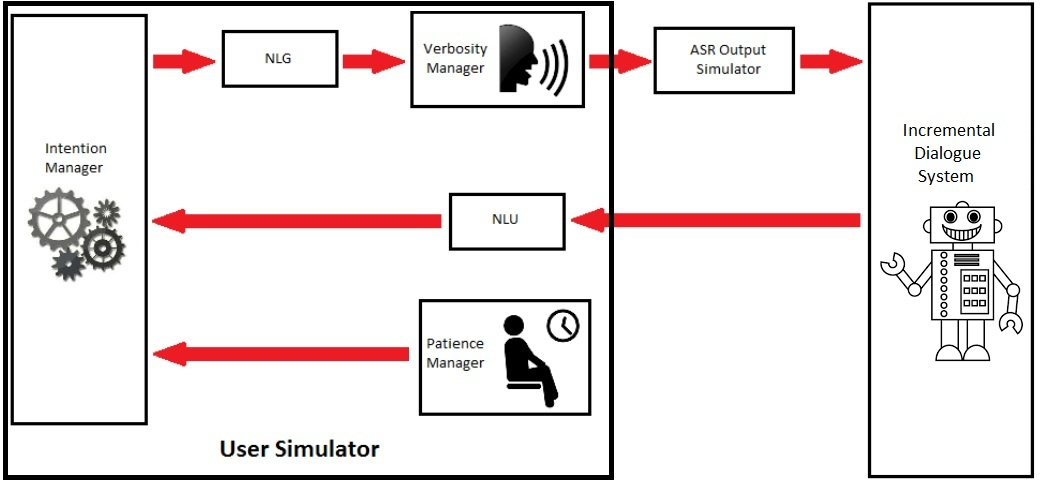
\includegraphics[scale=0.45]{figures/SimuSys.jpg}
			\caption{Simulated environment architecture}
			\label{fig:simuoverview}
		\end{figure*}
    
\section{User simulator}
	%\subsection{Overview}
    %
    	%The US is composed of five modules (see Figure \ref{fig:archi}). The Intent Manager, the NLU, the Verbosity Manager, the NLG and the Patience Manager. As discussed in Chapter \ref{ch:architecture}, in every incremental dialogue setup, each dialogue turn is divided into smaller micro-turn given a particular criteria; a micro-turn could be a time window (500 milliseconds for example), it could also be word-based or concept-based (a new word or a new concept marks the end of a micro-turn). The US described here is word-based.
        %
				
        %HK> Blinder un peu, c'est une simplification du barge-in human car rien ne garantit que la personne interrompue se taise.
        
				%At each micro-turn, the US generates a partial N-Best. It corresponds to the whole utterance from the beginning of the turn (\textit{restart incremental} mode \cite{Schlangen2011}). On the other hand, either the US receives an answer from the Scheduler at a certain micro-turn and it stops speaking, either it does not and it continues speaking if it has additional things to say (releasing the floor otherwise). When the dialogue lasts for too long without achieving the task at hand, the US can end the dialogue.
				%
        %
        %In the following, the different components of the US are described in detail.
        %
        %\begin{figure*}[htb]
          %\centering
          %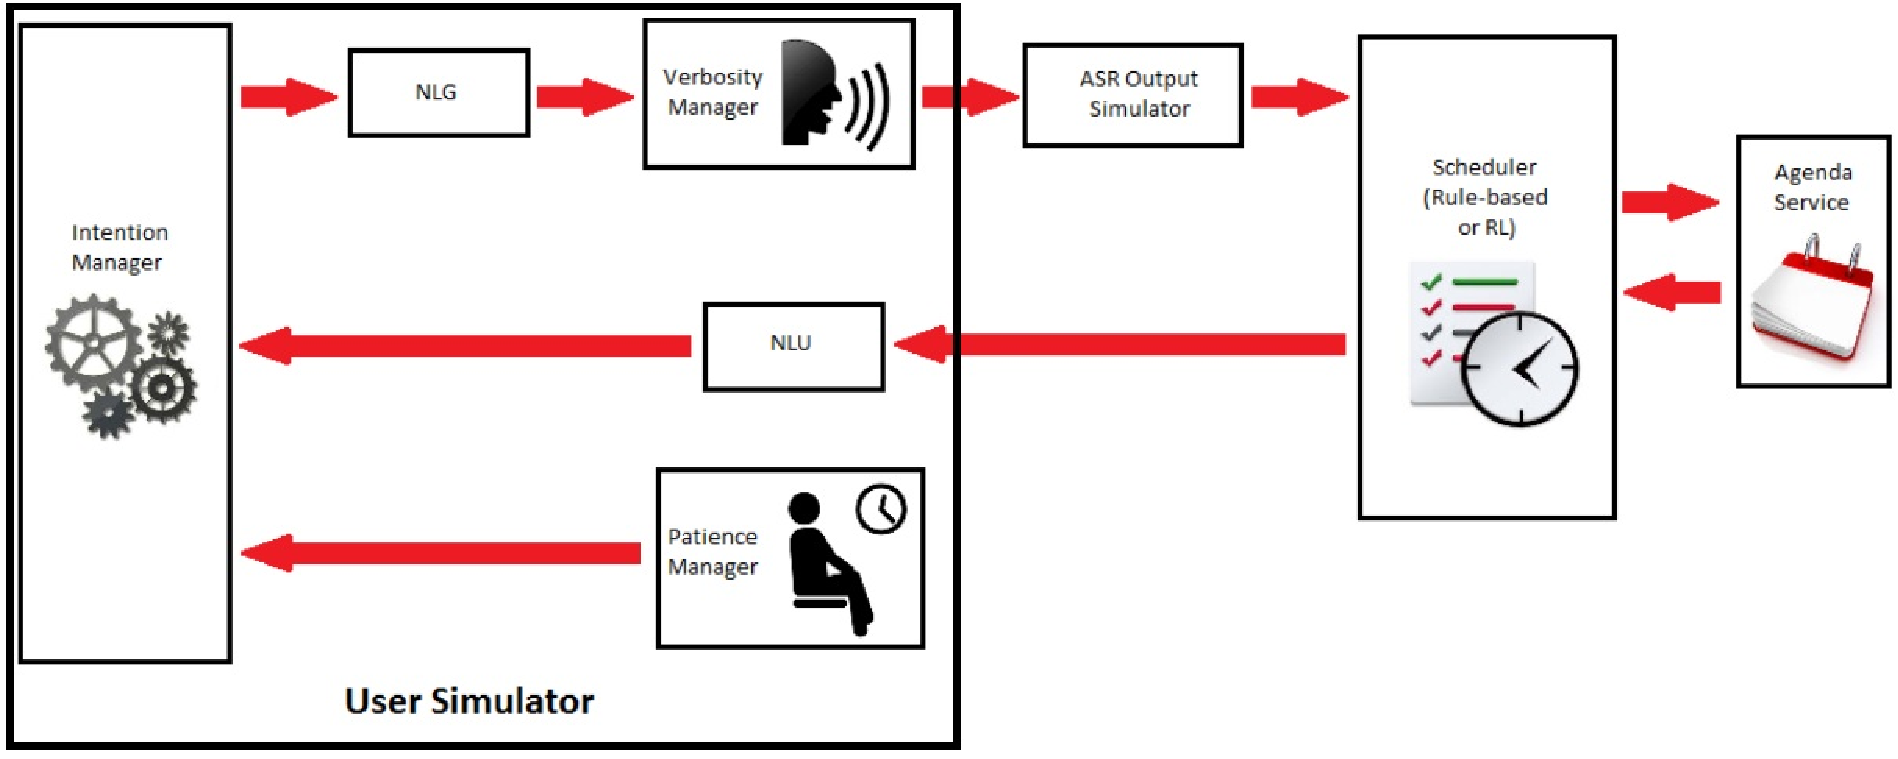
\includegraphics[scale=0.45]{figures/ArchiSimuSys.pdf}
          %\caption{Simulated environment architecture}
          %\label{fig:archi}
        %\end{figure*}
				
				In a nutshell, at the $p^{th}$ micro-turn of the $k^{th}$ user turn $\mu T^{k,U}_p$, the US generates a partial utterance $Req^k_p$ that is transformed into an N-Best ${(s^k_{p,1}, hyp^k_{p,1}),...,(s^k_{p,N}, hyp^k_{p,N})}$. It corresponds to the whole utterance pronounced during the partial turn $T^{k,U}_p$ (\textit{restart incremental} mode \cite{Schlangen2011}). On the other hand, either the US receives an answer from the dialogue system at a certain micro-turn and it stops speaking\footnote{This is of course an approximation of real barge-in cases since the overlap is neglected.}, either it does not and it continues speaking if it has additional things to say (releasing the floor otherwise). When the dialogue lasts for too long without achieving the task at hand, the US can end the dialogue.

                                In the following, the role and the functioning of the US and the ASR output simulator are discribed in an abstract fashion before being instanciated later on to give birth to a personal agenda management simulated environment.
    
\section{User Simulator}

    \subsection{Intent Manager}
    \label{subsec:intentmanager}

        The Intent Manager is in charge of computing the dialogue acts that the US performs. It maintains an internal dialogue context and takes the dialogue acts coming from the dialogue system as inputs. Thus, it can be viewed as a dialogue manager in itself but with the difference that it is aimed to generate requests and lead the dialogue instead of serving a user (at least in task-oriented situations). Therefore, it is given a task or a list of tasks to accomplish before it starts interacting with the dialogue system.

        A common approach to design such a module is the agenda-based method \cite{Wei1999,Schatzmann2007}. Inspired by the latter, the approach adopted in this thesis suggests that the tasks the Intent Manager should accomplish are given in the form of a stack (LIFO structure): \textit{actionStack}. They are removed and executed one by one and during each step, new actions could be added. The Algorithm \ref{alg:abstractim} describes a recursive function called \textit{act} that is given \textit{actionStack} and that is in charge of performing all the corresponding actions by using the method \textit{execute()}. The latter removes and tries to execute the top element of the action stack which might lead to the creation of new actions that are added on top of \textit{actionStack} (which justifies the fact that the whole stack is passed as an argument and not the top element only). Once it has finished its treatment, \textit{act} is called over the updated stack.

        \begin{algorithm}[htp]
          \DontPrintSemicolon
          \SetKwFunction{act}{act}
          \SetKwProg{myalg}{Algorith}{}{}
          \myalg{\act{actionStack}}{
            \If{actionStack not empty}{
              execute(actionStack)\;
              act(actionStack)\;
            }
          }
          \caption{Intent Manager abstract algorithm}
          \label{alg:abstractim}
        \end{algorithm}

        %The Intent Manager computes the next dialogue act made by the US given the current dialogue state and by using an agenda-based approach \cite{Wei1999,Schatzmann2007}: the Intent Manager uses a stack of actions that is updated during the dialogue. The US finishes the dialogue when that stack is empty. Here, the aim of the US is to make the biggest number possible of events with the highest priority values taken from \textit{InitList} and \textit{ToAddList} fit in the agenda. To do so, the Intent Manager recursively runs the act function (taking the action stack as an argument) depicted in Algorithm \ref{algo:intent} where
        
        %HK> Cf les remarques de Romain sur le premier draft IWSDS pour cette partie.
        
        %\begin{itemize}
         % \item \textbf{actionStack:} the stack\footnote{The top element of the stack is called actionStack.top and it is removed by calling actionStack.removeTop().} of actions to be performed by the system (initially the list of ADD actions corresponding to \textit{ToAddList}).
          %\item \textbf{act():} function that performs a list of actions.
          %\item \textbf{perform():} function that performs a single action.
          %\item \textbf{alternatives(action):} function that returns the alternative events that can be used to perform \textit{action}.
          %\item \textbf{conflictsByAlt:} contains couples (event,conflictSet) mapping events to the sets of conflicting events in the agenda.
          %\item \textbf{maxPrioByAlt:} contains couples (event, maxPrio) mapping events to the maximum priority in conflictsByAlt(event).
        %\end{itemize}
			
	%		\begin{algorithm}[htp]
        %      \DontPrintSemicolon
        %      \SetKwFunction{act}{act}
        %      \SetKwProg{myalg}{Algorithm}{}{}
        %      \myalg{\act{actionStack}}{
        %        \If{actionStack not empty}{
        %        	added $\gets$ perform(actionStack.top)\;
        %        	\If{not added}{
        %            	alt $\gets$ alternatives(actionStack.top)\;
        %                conflictsByAlt $\gets$ []\;
        %                maxPrioByAlt $\gets$ []\;
        %                addedAlt $\gets$ false\;
        %                \While{alt not empty AND not addedAlt}{
        %                	addedAlt $\gets$ perform(alt(0))\;
        %                    \If{not addedAlt}{
        %                    	conflictsByAlt $\gets$ [conflictsByAlt ; (alt(0),conflicts(alt(0)))]\;
        %                        maxPrioByAlt $\gets$ [maxPrioByAlt ; (alt(0),max priority of conflicts(alt(0)))]\;
        %                        alt.remove(0)\;
        %                    }
        %                }
        %                
        %                \If{not addedAlt}{
        %                	selectedAlt $\gets$ argmin maxPrioByAlt\;
        %                    movedToAlt $\gets$ true\;
        %                    \While{conflictsByAlt no empty AND movedToAlt}{
        %                    	moveActionStack $\gets$ stack of move actions to the different alternatives of conflict\;
        %                        movedToAlt $\gets$ act(moveActionStack)\;
        %                    }
        %                    \uIf{movedToAlt}{
        %                    	perform(ationStack.top)\;
        %                    }
        %                }
        %            }
        %            
        %            actionList.removeTop()\;
        %            act(actionStack)\;
        %        }
        %      }{}
        %      \caption{Intent Manager algorithm}
        %      \label{algo:intent}
        %  	\end{algorithm}
    
    \subsection{NLG and Verbosity Manager}
		
			The NLG module transforms action concepts as well as date, time window, description and yes/no concepts into simple straightforward utterances. For instance the NLG result for the intent ACTION(ADD, EVENT(birthday party, DATE(6,1), WINDOW(TIME(21,0), \\ TIME(23,0)))) is \textit{add the event birthday party on January $6^{th}$ from 9pm to 11pm}.
			
			Nevertheless, compared to human/human conversations, limiting interactions to this kind of simple utterances is not realistic. Therefore, they are enhanced in the Verbosity Manager with prefixes like \textit{I would like to}, \textit{Is it possible to}...and suffixes like \textit{if possible}, \textit{please}... In \cite{Ghigi2014}, a corpus study showed that users tend to go off-domain and to repeat the same information several times in the same sentence. These behaviours are also replicated in the Verbosity Manager: 10\% of the times, the US utters an off-domain sentence, and 30\% of the times where there is a misunderstanding, it repeats the same information twice.
		
    \subsection{ASR output simulator}
    \label{subsec:asroutputsimu}
		
			\begin{figure*}[hb]
          \centering
          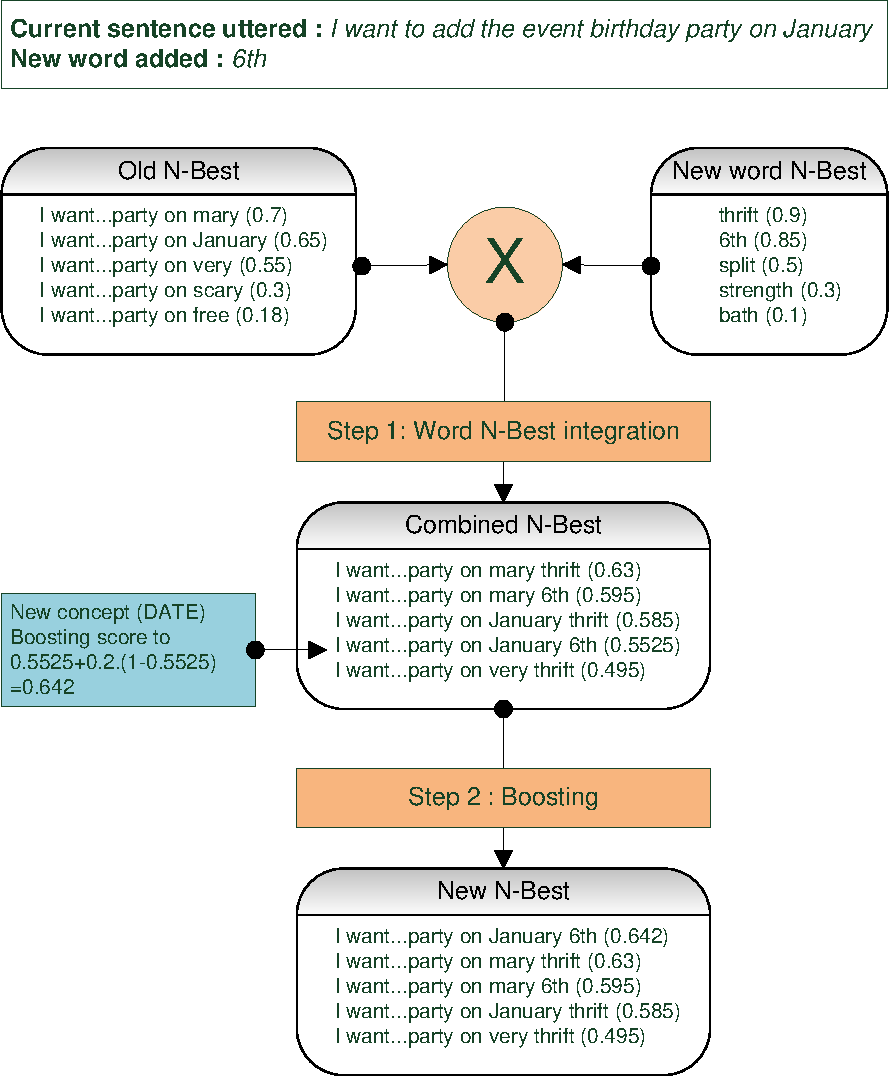
\includegraphics[scale=0.8]{figures/ASRSimu.pdf}
          \caption{An illustration of the incremental ASR output N-Best update}
          \label{fig:asrsimu}
        \end{figure*}
    
     	The ASR output simulator generates an N-Best that is updated at each new micro-turn. For instance, if at a certain point, the US uttered \textit{I would like to add the event birthday party on...}, a possible N-Best could be (the numbers between brackets represent ASR scores):
        
        \begin{itemize}
					\item (0.82) I would like to add the event birthday party on
					\item (0.65) I like to add the event birthday party on
					\item (0.43) I have had the event birthday party
					\item (0.33) I would like to add the holiday party
					\item (0.31) I like to add the holiday party on
        \end{itemize}
        
       	More formally, at time t, the N-Best is an N-uplet ${(s_1^{(t)},hyp_1^{(t)}),...,(s_N^{(t)},hyp_N^{(t)})}$. At time t+1, a new word $w_{t+1}$ is sent to the ASR output simulator and the latter calculates a new associated N-Best. Therefore, at this stage, the system has two N-Bests:
				
				\begin{itemize}
					\item \textbf{The word N-Best:} It corresponds to the different hypotheses related to the last word pronounced. In Figure \ref{fig:asrsimu}, the top right box represents the word N-Best associated with the word $6^{th}$.
					\item \textbf{The utterance N-Best:} It designates the N-Best associated with the whole partial utterance pronounced so far. In Figure \ref{fig:asrsimu}, the top left box is an a example of such N-Best associated with the partial utterance \textit{I want to add the event birthday party on January}.
				\end{itemize}
				
				Both are combined to form the new utterance N-Best. In the following, the way the word N-Best is calculated and the way it is incorporated into the partial utterance N-Best are described.
				
				In order to simulate noise and ASR imperfections, the ASR output simulator uses a module called the Scrambler. It receives a word as input and performs ones of the three following operations in order to compute the ouptut\footnote{Like most of the parameters, in this chapters, the values given here are empirical and they can be changed to model several configurations.}:
				
				\begin{itemize}
					\item Replace the word with a different word taken randomly from a dictionary (probability: 0.7).
					\item Add a new word (probability : 0.15).
					\item Delete the word (probability : 0.15)
				\end{itemize}
        
        A Word Error Rate (WER) is given as a parameter to the ASR output simulator. It controls the noise level that one wants to simulate. The algorithm used to generate the N-Best associated with a single word is described below:
        
        %HK> Citer le papier d'Olivier et de Richard Beaufort sur la simulation d'ASR en rapport avec ce graph.
        
        \begin{figure}[t]
				\centering
				\begin{tikzpicture}[scale=0.8]
				\begin{axis}[
					xlabel={Score},
					ylabel={Density},
					scaled ticks = false,
					tick label style={/pgf/number format/fixed},
					xmin=0, xmax=1,
					ymin=0, ymax=0.55,
					xtick={0,0.2,0.4,0.6,0.8,1},
					ytick={0.1,0.2,0.3,0.4,0.5,0.6},
                    legend pos=north east,
					ymajorgrids=true,
					grid style=dashed,
                    colorbrewer cycle list=Set2,
				]
				
				\addplot+[
					error bars/.cd,
					y dir=both,
					y explicit,
					]
					coordinates {
					(0,0)
(0.1,0.19483312081792062)
(0.2,0.3702598583755481)
(0.3,0.3943180330023535)
(0.4,0.33431406881442405)
(0.5,0.24197072451914337)
(0.6,0.1485840305841884)
(0.7,0.07242576116369753)
(0.8,0.023141241148471745)
(0.9,0.00240534717059161)
(1,0)
					};
                    
                    \addplot+[
					error bars/.cd,
					y dir=both,
					y explicit,
					]
					coordinates {
					(0,0)
(0.1,0.002405347170591614)
(0.2,0.023141241148471745)
(0.3,0.0724257611636976)
(0.4,0.14858403058418854)
(0.5,0.24197072451914337)
(0.6,0.33431406881442416)
(0.7,0.3943180330023536)
(0.8,0.37025985837554803)
(0.9,0.1948331208179205)
(1,0)

					};
                    

				\legend{Bad recognition,Good recognition}

				\end{axis}
				\end{tikzpicture}
				\caption{ASR score sampling distribution}
				\label{fig:scoresample}
		\end{figure}
    
        \begin{enumerate}
        	\item Determine whether $w_{t+1}$ is among the N-Best or not with a probability that is computed as follows: (1 - WER) + INBF.WER, where INBF (In N-Best Factor) is a parameter between 0 and 1 (set to 0.7 in this thesis). If $w_{t+1}$ is not in the N-Best, then the latter contains only scrambled versions of this word and jump to step 4.
            \item The first hypothesis is set to be $w_{t+1}$ with a probability of (1-WER), otherwise, it is a scrambled version of it.
            \item If the the first hypothesis is not $w_{t+1}$, then this word's position is randomly chosen between 2 and N. Moreover, the other hypothesis are scrambled versions of it.
            \item The confidence score associated with the best hypothesis ($s_0$) is sampled as sigmoid(X) where X is a gaussian and
						
						\begin{eqnarray}
							sigmoid(x) & = & \frac{1}{1 + e^{-x}}
						\end{eqnarray}
						
						More precisely, $X \sim \mathcal{N} (-1,1)$ if the first hypothesis is wrong and $X \sim \mathcal{N} (1,1)$ when it is right. The standard deviation of X is one. By taking the sigmoid, this leads to two distributions\footnote{Confidence score estimation is a complex problem and it is still a research topic \cite{Jiang2005,Seigel2011}. The simple model introduced here is inspired by \cite{Pietquin2005}. Also, notice that the scores are between 0 and 1 but they do not sum up to 1 since they are not probabilities.} (depicted in Figure \ref{fig:scoresample}) with a mean of 0.3 and 0.7 and a standard deviation of 0.18 for both (which can be changed to simulate different levels of accuracy of the confidence score model. The closest to 0, the more discriminative the model).
            \item The scores for the other hypotheses are computed in an iterative way. For $i$ between 2 and N, $s_i$ is uniformly sampled in $[0,s_{i-1}]$.
        \end{enumerate}
        
        In incremental settings, the ASR input is a continuous audio stream. In reality, it is split into small consecutive chunks of data. At each new input arrival, the output is updated. However, a new chunk of audio data in the input does not necessarily translate into a new chunk of text added to the output. In reality, the latter can be partially or even completely changed while update. An example from \cite{Schlangen2011} is when the user utters the word \textit{forty}: the system first understands \textit{four} and then \textit{forty}. The transition between the two hypotheses does not translate into an addition of information but the first hypothesis has to be revoked and replaced by the second one. This phenomenon is referred to as the \textit{ASR instability}.
        
        As already mentioned in this thesis, early partial utterances are not necessarily prefixes of later ones (ASR instability phenomenon). To replicate this behaviour, a language model is needed to compute the scores corresponding to the different hypotheses in the N-Best. Therefore, sentences that are more in alignment with the model have higher scores thus being pushed to the top of this N-Best. Here, the NLU knowledge is used as a proxy for the language model by making the following assumption: \textit{the more an utterance generates key concepts once fed to the NLU, the more it is likely to be the correct one}. Therefore, as soon as a new action, date or time window concept is detected in $hyp_i$, $s_i$ is boosted as follows:
        
        	$$ s_i \leftarrow s_i + BF.(1 - s_i) $$
            
      	where BF is the Boost Factor parameter. Here it is set to 0.2. An illustration of this mechanism is provided in Fig. \ref{fig:asrsimu}.
    
    \subsection{Timing and patience manager}
    
    	When it comes to incremental processing, timing is key. However, the main objective of simulation is to generate dialogues in an accelerated mode, hence, no track of timing is kept. In order to approximate durations, the user's and the system's speech rates are considered to be 200 words per minute \cite{Yuan2006}.
        
        Users tend to get impatient, at various degrees, when dialogue systems take too long to accomplish the task they are asked for. To simulate this behaviour, a duration threshold is chosen at each new dialogue that will cause the user to hangup as soon as it is reached. It is computed as follows
        
       	\begin{eqnarray}
        	d_{pat} = 2 \mu_{pat}.sigmoid(X)
        \end{eqnarray}
        
        where X follows a gaussian distribution of mean 0 and variance 1 and consequently $\mu_{pat}$ is the mean duration threshold (here, $\mu_pat = 180 s$).
    
